\startchapter{Evaluation, Analysis and Comparisons}
\label{chapter:evaluation}
Our methods presented in the previous chapters have been integrated into our surgical simulation system. 
The result is a comprehensive environment for soft-tissue modeling and simulation with support for cutting and
probing. We present our results in the context of two procedures.

The first operation is craniotomy which is a surgical operation in which a bone flap is temporarily removed 
from the skull to access the brain. Craniotomies are often a critical operation performed on patients suffering 
from brain lesions or traumatic brain injury (TBI), and can also allow doctors to surgically implant deep brain 
stimulators for the treatment of Parkinson's disease, epilepsy and cerebellar tremor. The procedure is also widely 
used in neuroscience for extracellular recording, brain imaging, and for neurological manipulations such as electrical 
stimulation and chemical titration. Craniotomies are also named according to their size and complexity. Small dime-sized 
craniotomies are called burr holes or keyhole craniotomies. Sometimes stereotactic frames, image-guided computer systems, 
or endoscopes are used to precisely direct instruments through these small holes. Burr holes or keyhole craniotomies are 
used for minimally invasive procedures to:

\begin{itemize}
 \item insert a shunt into the ventricles to drain cerebrospinal fluid (hydrocephalus)
 \item insert a deep brain stimulator to treat Parkinson Disease
 \item insert an intracranial pressure (ICP) monitor
 \item remove a small sample of abnormal tissue (needle biopsy)
 \item drain a blood clot (stereotactic hematoma aspiration)
 \item insert an endoscope to remove small tumors and clip aneurysms
\end{itemize}


The second simulation operation is brain biopsy which is the removal of a small piece of brain tissue for the diagnosis of abnormalities 
of the brain. It is used to diagnose Alzheimer's disease, tumors, infection, inflammation, and other brain disorders. By examining 
the tissue sample under a microscope, the biopsy sample provides doctors with the information necessary to guide diagnosis and 
treatment.

\section{Craniotomy}
Fang \etal published a tetrahedral mesh data-set of the brain tissues \cite{fang2010mesh}. The MRI scanned data is 
segmented into the following four regions:

\begin{enumerate}
 \item Skull and scalp
 \item Cerebro-spinal fluid (CSF)
 \item Gray-matter
 \item White-matter
\end{enumerate}

The high-resolution version of these segments are not published at the time of this writing so we used the lower resolution 
which has enough details of the organ for our simulation scenarios. The data-set is converted from its original format 
(MATLAB mat file) to our volumetric mesh format. Table \ref{table:brainmesh} shows number of nodes, edges, faces and tetrahedral cells 
per each segment after the conversion process:

\begin{table}[H]
\begin{center}
\caption{\label{table:brainmesh}{Segmented brain data-set statistics.}}
  \begin{tabular}{ | l | c | c | c | c |}
    \hline    
     & skull & csf & gray matter & white matter \\ \hline \hline    
    Nodes & 14739 & 37136 & 50741 & 23737  \\ \hline
    Edges & 89681 & 181593 & 268300 & 126441 \\ \hline
    Faces & 141498 & 251823 & 384989 & 184536 \\ \hline
    Cells & 66554 & 107460 & 167528 & 81833 \\ \hline
    \hline
  \end{tabular}
\end{center}
\end{table}

Due to its stiff material properties the skull tissue is modelled as a rigid material in our simulation system. 
Figure \ref{fig:craniotomy01} shows the skull mesh in its initial position.

\begin{figure}[H]
  \centering
  % the following command controls the width of the embedded PS file
  % (relative to the width of the current column)
  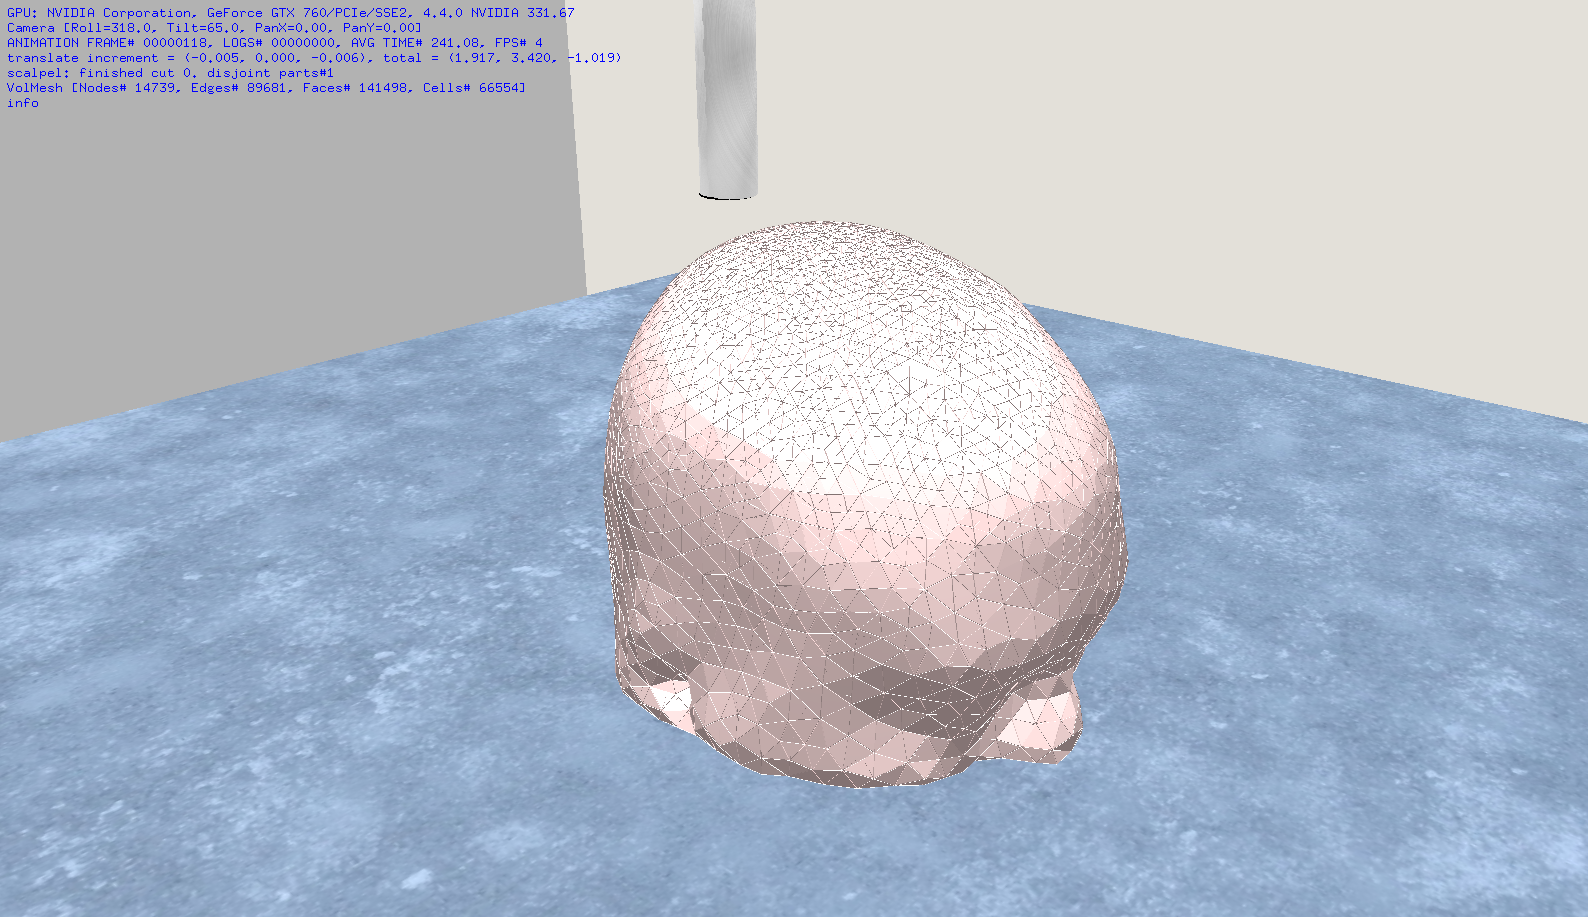
\includegraphics[width=0.7\linewidth]{figures/evaluation/craniotomy01.png}
  \caption{\label{fig:craniotomy01}
  {The scene setup for the craniotomy operation.}
}
\end{figure}


The cutting tool in this scenario is a tube-shaped device which can drill into the skull tissue and separate the bone matter.
In our system, the tool is defined as a curve approximated by $N$ line segments. The tool movement is tracked in the space 
and the system checks for collisions between the tool and the model constantly. Figure \ref{fig:craniotomytube} shows the 
polygonal shape of the cutting tool while in contact with the skull tissue.

\begin{figure}[H]
  \centering
  % the following command controls the width of the embedded PS file
  % (relative to the width of the current column)
  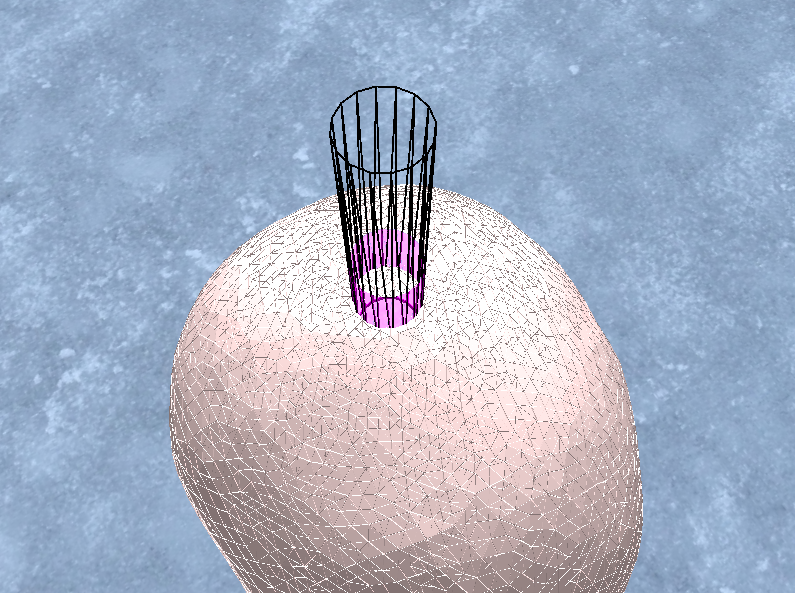
\includegraphics[width=0.6\linewidth]{figures/evaluation/craniotomytube.png}
  \caption{\label{fig:craniotomytube}
  {Cutting tool is defined as a tube with a base composed of a curve approximated with $N$ line segments. 
  Collisions between the tool and the tissue are monitored constantly.}
}
\end{figure}

When in contact with the skull tissue the intersection of the side wall of the tool is computed against the edges of the 
skull model. With $N$ line segments the cutting tool has $N$ quadrilateral faces on its side wall, the edge intersection 
test is performed in our system by calling the kernel function given in algorithm \ref{alg:edgeIntersections} once per each quad.
After each call the hash-table storing the cut-edges is filled with the new cuts. In case an edge is cut twice by the tool only 
the first cut is retained. This situation happens when a long edge of the tissue model is cut by relatively shorter segments of 
the cutting tool which is also illustrated in figure \ref{fig:ringscalpalissue}.

\begin{figure}[H]
  \centering
  % the following command controls the width of the embedded PS file
  % (relative to the width of the current column)
  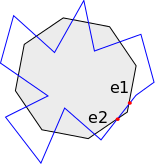
\includegraphics[width=0.2\linewidth]{figures/evaluation/ringscalpalissue.png}
  \caption{\label{fig:ringscalpalissue}
  {An edge in the volumetric mesh model is cut by multiple segments of the scalpel (Intersection points are shown in red dots)
   Only the first intersection is accepted in this case.}
}
\end{figure}


The cutting configurations presented in section \ref{sec:cutconfigs} are extracted based on one intersection per edge, therefore
it's not possible to cut a given edge more than once. In our system we only accept the first cut-edge and this did not produce any 
visual defects. Perhaps a more robust implementation would be to approximate the cutting tool curve based on the size of the longest 
edge in the mesh. After the cutting is made the mesh is separated and each of the disconnected parts is converted into a separate node
in our scenegraph structure. This operation results in correct detection of the self-collisions in the subsequent frames of the simulation.

The internal gray, white and CSF matters are also included in this simulation. The drilling operation only affects the skull tissue and
in fact it does not pass the Dura layer. This condition is a requirement for the successful completion of this procedure. 

Figure \ref{fig:crosssection} shows the cross section view of the brain. The skull is cut with a scalpel tool 
to show the internal tissues which are drawn in blue for better visibility. 
\begin{figure}[H]
  \centering
  % the following command controls the width of the embedded PS file
  % (relative to the width of the current column)
  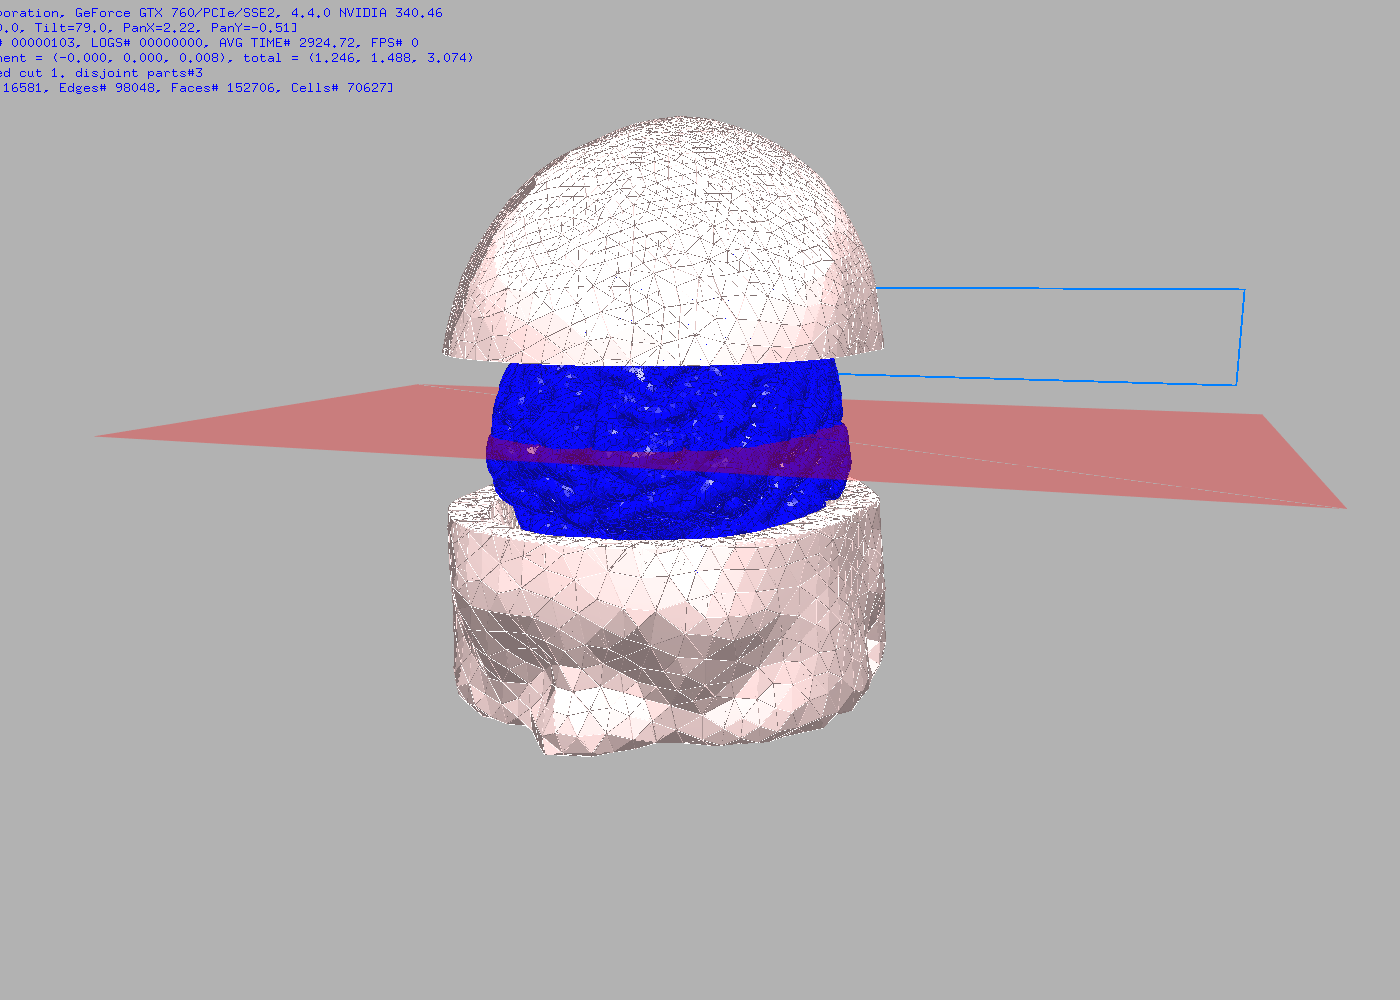
\includegraphics[width=0.5\linewidth]{figures/evaluation/crosssection.png}
  \caption{\label{fig:crosssection}
  {Cross section view of the brain layers. The skull shown in pink is cut using a scalpel avatar to show 
   all the other layers depicted in blue.}
}
\end{figure}

\begin{figure}[H]
  \centering
  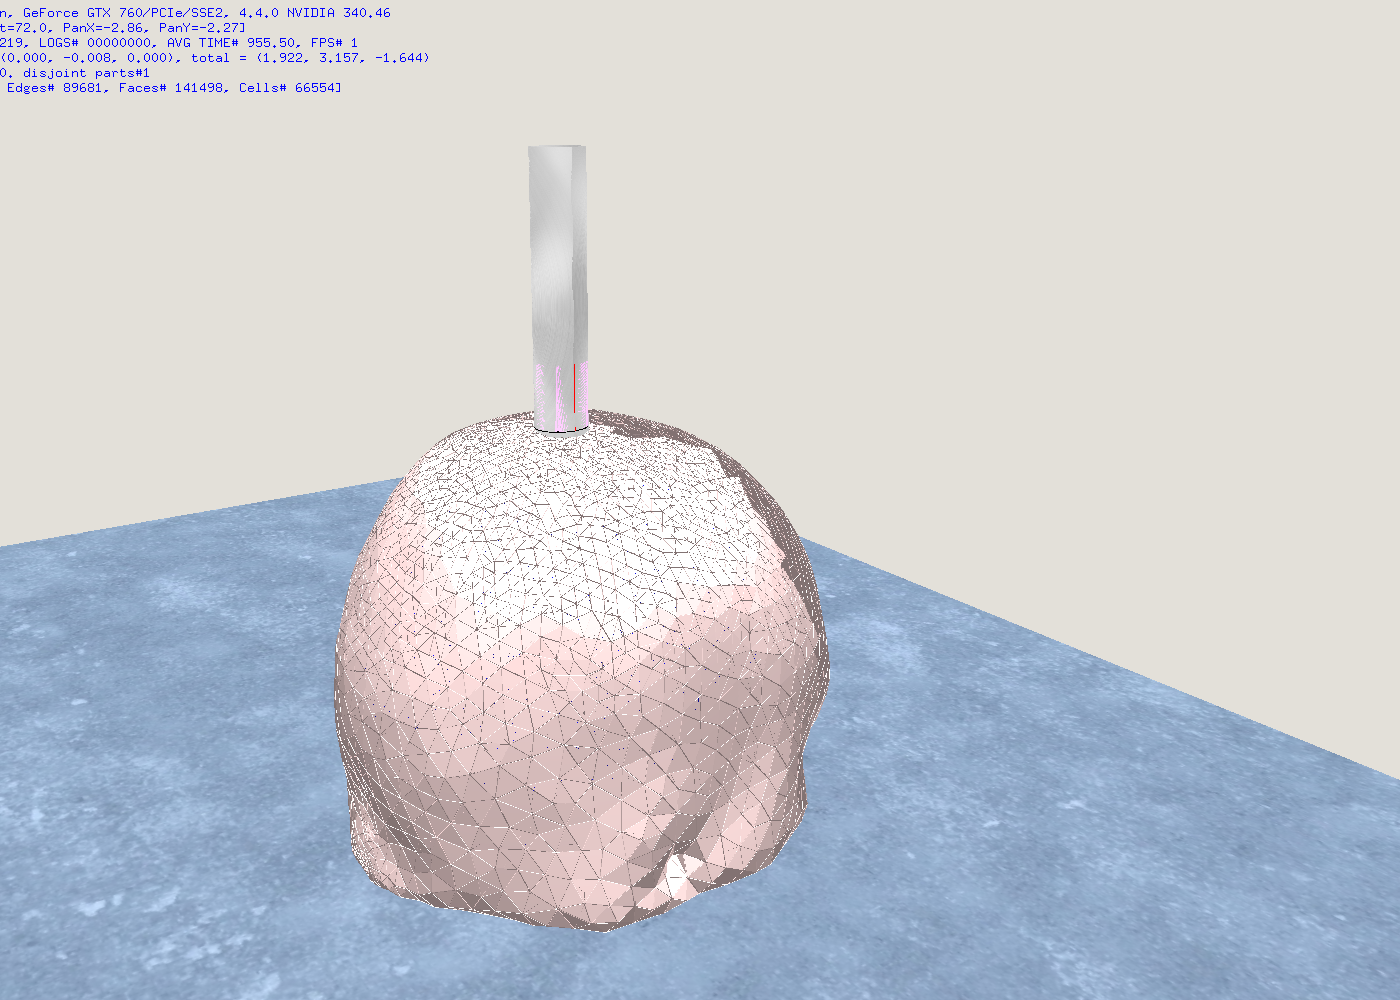
\includegraphics[width=0.5\linewidth]{figures/evaluation/craniotomy06.png}
  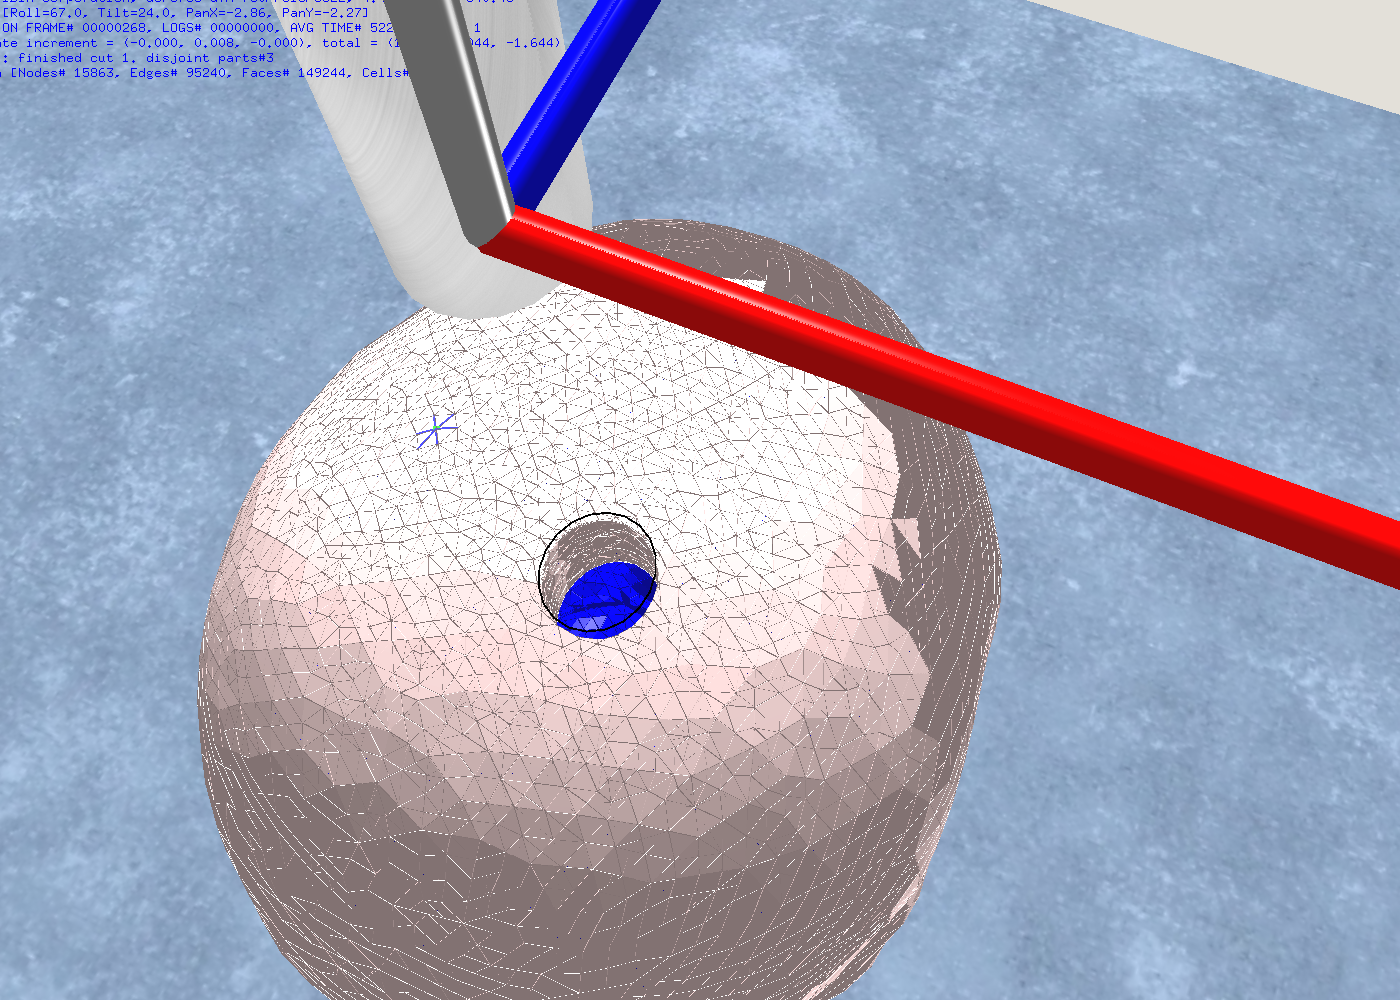
\includegraphics[width=0.5\linewidth]{figures/evaluation/craniotomy07.png}
  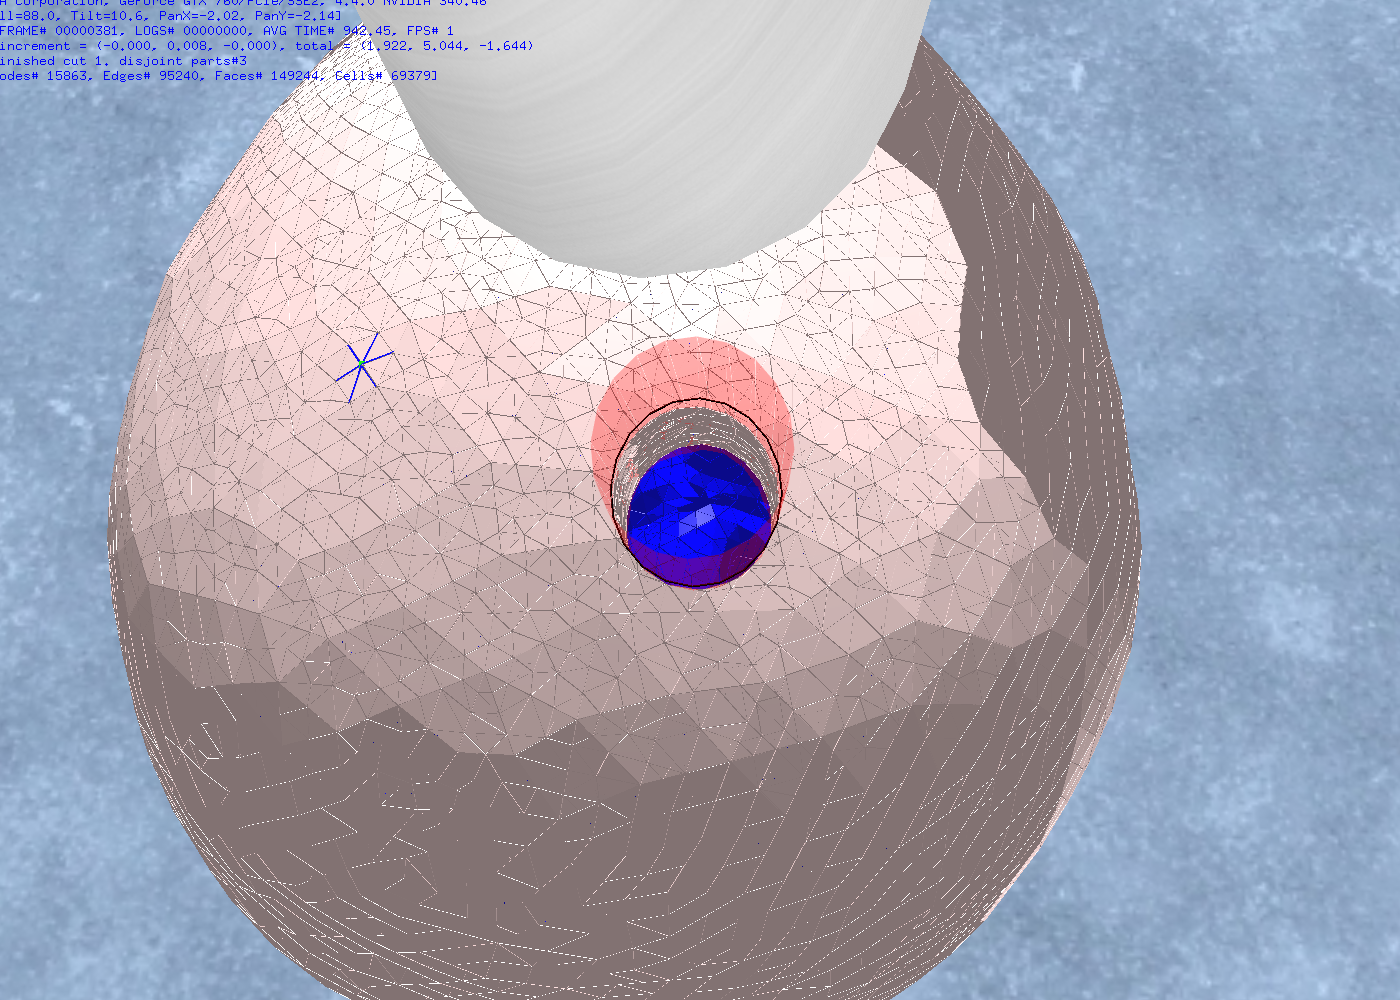
\includegraphics[width=0.5\linewidth]{figures/evaluation/craniotomy08.png}
  \caption{\label{fig:craniotomy}
  {Simulation of the craniotomy operation using our surgical simulation framework with support for interactive cutting.}
}
\end{figure}

Figure \ref{fig:craniotomy} shows the three stages of the operation (before, during and after the cutting operation). 
During the drilling process 845 tetrahedral cells are being cut in the vicinity of the drilling tool. 